% import packages
\documentclass[12pt,a4paper]{article}
\usepackage{varwidth}
\usepackage{multicol}
\usepackage{booktabs}
\usepackage{threeparttable}
\usepackage{enumitem}
\usepackage{algorithm}
\usepackage{algpseudocode}
\usepackage{ragged2e}
\usepackage[hidelinks]{hyperref}
\usepackage[font=footnotesize]{caption}
\usepackage{csquotes}
\usepackage{float}
\usepackage[round,sort]{natbib}
\usepackage{tikz}
\usepackage{listings}
\usetikzlibrary{arrows,positioning,decorations.pathreplacing,shapes,calc,fit}
\usepackage{lipsum}
\usepackage{amsmath}
\usepackage{amssymb}
\usepackage{geometry}
\usepackage{url}
\usepackage{array,tabularx}

% define global latex variables
\renewcommand{\algorithmicrequire}{\textbf{Input:}}
\renewcommand{\algorithmicensure}{\textbf{Output:}}
\captionsetup[algorithm]{labelsep=colon}
\algnewcommand\algorithmicforeach{\textbf{for each}}
\algdef{S}[FOR]{ForEach}[1]{\algorithmicforeach\ #1\ \algorithmicdo}
\geometry{top=2.5cm,
		bottom=2.5cm}
\graphicspath{{img/}}
\newcommand\BibTeX{B\textsc{ib}\TeX}
%\renewcommand{\contentsname}{Table of Contents}
%\renewcommand{\refname}{Bibliography}
\newcolumntype{L}[1]{>{\RaggedRight\hspace{0pt}}p{#1}}
\newcolumntype{R}[1]{>{\RaggedLeft\hspace{0pt}}p{#1}}
\captionsetup[figure]{font=footnotesize,labelfont=footnotesize,labelfont={bf},labelformat={default},labelsep=period,name={Fig.}, justification=centering,singlelinecheck=false, width = \linewidth}
\captionsetup[table]{font=footnotesize,labelfont=footnotesize,labelfont={bf},labelformat={default},labelsep=period,name={Table},justification=centering, singlelinecheck=false, width = \linewidth}

% define global tikz variables
% From http://tex.stackexchange.com/questions/123760/draw-crosses-in-tikz
\tikzset{cross/.style={cross out, draw=black, fill=none, minimum size=15pt, inner sep=0pt, outer sep=0pt}, cross/.default={2pt}}
\tikzset{pblock/.style = {rectangle split, rectangle split horizontal,
                      rectangle split parts=2, very thick,draw=black!60,fill=black!7, align=center}}
\tikzset{recBlock/.style = {rectangle,very thick,draw=black!60,fill=black!7,align=center,
                      minimum width = 3cm, minimum height = 2cm,
                      text width = 2.5cm}}
\tikzset{recBlock2/.style = {rectangle,very thick,draw=black!60,fill=black!7,align=center,
                      minimum width = 2.5cm, minimum height = 2cm,
                      text width = 2.5cm}}
\tikzset{vblock/.style = {rectangle,very thick,draw=black!60,  fill = red!20, align=center,minimum width = 3.5cm, minimum height = 4cm,text width = 3.5cm}}
\tikzset{vblock2/.style = {rectangle,very thick,draw=black!60,  fill = red!20, align=center,minimum width = 4cm, minimum height = 2.5cm,text width = 3.5cm}}
\tikzset{vblock3/.style = {rectangle,very thick,draw=black!60,  fill = red!20, align=center,minimum width = 8cm, minimum height = 3cm,text width = 8cm}}
\tikzset{vblock4/.style = {rectangle,very thick,draw=black!60,
                      fill=red!20,align=center,
                      minimum width = 2.5cm, minimum height = 2cm,
                      text width = 2.5cm}}
\tikzset{
    %Define standard arrow tip
    >=stealth',
    % Define arrow style
    pil/.style={
           ->,
           thick,
           shorten <=2pt,
           shorten >=2pt}
}
\tikzset{
    %Define standard arrow tip
    >=stealth',
    % Define arrow style
    pil2/.style={
           ->,
           thick,
           shorten >=2pt}
}

% define admin variables
\title{Investigating the Utility of Answer Set Programming and Inductive Logic Techniques in Learning Two-Player Game Strategies}
\author{Susana Hahn, Atreya Shankar\\
\texttt{\{hahnmartinlu,shankar\}@uni-potsdam.de} \\
PM: Computational Intelligence, WiSe 2019/20 \\
Prof. Dr. Torsten Schaub \\
Research Group: Knowledge Processing and Information Systems \\
Institute of Computer Science, University of Potsdam}
\date{\today}

\begin{document}
\newgeometry{}
\maketitle
\thispagestyle{empty}
\begin{abstract}
In the last decades, significant advancements have been made in optimizing artificially intelligent computer agents in two-player games. In this project, we aim to learn strategies from games encoded in Game Description Language (GDL) while simulating the gameplay using Answer Set Programming (ASP) in \textit{clingo}. We reformulate two common games, specifically \textit{Nim}, and \textit{Tic-Tac-Toe} and implement various techniques for learning explainable strategies. These approaches include flavours of the \textit{Minimax} algorithm to generate not only optimum decision trees but also ASP rules. Further, we use Inductive Learning Programming and the framework \textit{ILASP} to learn weak constraints from ordered examples. Finally, we benchmark the various learning techniques against one another in order to evaluate their effectiveness and scalability into bigger game instances. We were able to find strategies in the form of logic rules easily interpretable by humans. Our method represents a novel technique since we attempt to extend the utility of ASP from its traditional single-agent problem-solving setting to that of a dynamic dual-agent simulation setting. 
\end{abstract}
\newpage
\thispagestyle{empty}
\tableofcontents
\newpage
\restoregeometry
\setcounter{page}{1}
\thispagestyle{plain}
\section{Introduction}

In the last decades, significant advancements have been made in optimizing artificially intelligent computer agents in two-player games such as \textit{Chess} and \textit{Go} \citep{Silver1140}. Much of this success can be attributed to advancements in deep reinforcement learning and corresponding GPU hardware-acceleration \citep{Silver1140}. However, one common disadvantage of these techniques is the lack of explainability of the strategies learned; which is largely due to the black-box nature of deep learning models \citep{DBLP:journals/corr/abs-1804-02477}. These models are specially designed for games with a high branching factor which makes it impossible to explore the complete game space to make a decision. Most of these systems rely on Monte Carlo Tree Search and Reinforcement learning techniques to avoid the construction of a full search tree. In the case of smaller games, where we are able to compute the full tree search for smaller instances, more algorithms become available to perform the analysis.

In this project, we aim to learn game strategies for two common small games, specifically \textit{Nim}, and \textit{Tic-Tac-Toe}. We use formalisms from Game Description Language (GDL) \citep{love@ggp} to encode the rules of the games in Answer Set Programming (ASP)\citep{GlimpsASP}, and simulate the gameplay using the ASP system \textit{clingo}. We implement various techniques for learning game strategies; a brute force \textit{Minimax} algorithm, a specialized Minimax algorithm employing the optimization statements provided by \textit{clingo} and we also use Inductive Learning of Answer Set Programs (\textit{ILASP}) to learn weak constraints from positive ordered examples. Finally, we benchmark the various learning techniques against one another by treating them as independent agents to evaluate their performance and scalability. Our method represents a novel technique since we attempt to extend the utility of ASP from its traditional single-agent problem-solving setting to that of a dynamic dual-agent simulation setting.

In sections \hyperref[back_con]{2} and \hyperref[methods]{3}, we describe the aforementioned background concepts and methodologies respectively. In section \hyperref[results]{4}, we describe the results of our methodologies and then in section \hyperref[discussion]{5} proceed to discuss pertinent limitations of the tested methodologies. Finally, we conclude our research in section \hyperref[conclusions]{6}.
\section{Background Concepts}
\label{back_con}

\subsection{Our Two-Player Games}
\label{gameDescriptions}

\subsubsection{Nim}
\label{nim}

Nim is an old and well-known two-player game, which is rumored to have originated in China \citep{bouton1901nim}. Nim consists of a configuration of $N$ piles where each pile $i$ consists of $N_i$ objects; which are typically referred to as counters. During each round, a single player must take at least one counter from a single pile. The players play alternately and in the normal version of the game, the player who takes the last counter(s) wins. The game is usually played with four piles with initial counters $(7,5,3,1)$.
Since Nim has no draws, there is always a clear winning strategy for one of the players. Such a strategy is based on performing a binary digital sum, called \textit{Nim Sum}, representing the counters of each heap in binary and adding each unit individually. The key is to make sure you always leave the next player in a configuration where the \textit{Nim Sums} for every digit are even. In Figure ~\ref{fig:nim_sample} we can notice how player B uses this strategy and leaves piles with an even \textit{Nim Sums} for every digit, unlike the moves performed by player A.

\begin{figure}[H]
\centering
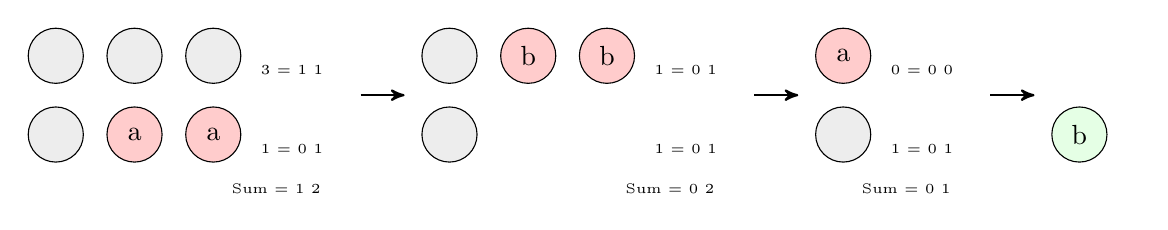
\begin{tikzpicture}
\filldraw[fill=black!7] (0,1) circle (0.35cm) node {};
\filldraw[fill=red!20] (1,1) circle (0.35cm) node {a};
\filldraw[fill=red!20] (2,1) circle (0.35cm) node {a};
\node[below, font=\tiny] at (3,1) {1 = 0 1};
\filldraw[fill=black!7] (0,2) circle (0.35cm) node {};
\filldraw[fill=black!7] (1,2) circle (0.35cm) node {};
\filldraw[fill=black!7] (2,2) circle (0.35cm) node {};
\node[below, font=\tiny] at (3,2) {3 = 1 1};

\node[below, font=\tiny] at (2.8,0.5) {Sum = 1 2};


\draw[pil] (3.8,1.5) -- node [above, text width = 3cm, align=center] {} (4.5,1.5);

\filldraw[fill=black!7] (5,1) circle (0.35cm) node {};
\node[below, font=\tiny] at (8,1) {1 = 0 1};

\filldraw[fill=black!7] (5,2) circle (0.35cm) node {};
\filldraw[fill=red!20] (6,2) circle (0.35cm) node {b};
\filldraw[fill=red!20] (7,2) circle (0.35cm) node {b};
\node[below, font=\tiny] at (8,2) {1 = 0 1};

\node[below, font=\tiny] at (7.8,0.5) {Sum = 0 2};


\draw[pil] (8.8,1.5) -- node [above, text width = 3cm, align=center] {} (9.5,1.5);

\filldraw[fill=black!7] (10,1) circle (0.35cm) node {};
\node[below, font=\tiny] at (11,1) {1 = 0 1};

\filldraw[fill=red!20] (10,2) circle (0.35cm) node {a};
\node[below, font=\tiny] at (11,2) {0 = 0 0};

\node[below, font=\tiny] at (10.8,0.5) {Sum = 0 1};

\draw[pil] (11.8,1.5) -- node [above, text width = 3cm, align=center] {} (12.5,1.5);

\filldraw[fill=green!10] (13,1) circle (0.35cm) node {b};


% \draw [decorate,decoration={brace,amplitude=10pt},xshift=-3pt,yshift=0pt,thick] (10.0,2.5) -- (10.0,0.5) node [black,midway,xshift=2cm,align=center, text width = 3cm] {Player \textbf{a} takes last counters and wins};
\end{tikzpicture}
\caption{Sample game of \textit{Nim} with a 2-pile starting configuration where player B wins by taking last counter; red indicates counter(s) taken. The binary representation is always done wrt the piles left.} 
\label{fig:nim_sample}
\end{figure}

% \begin{figure}[H]
%     \centering
%     \fbox{
%     \includegraphics[width=0.5\columnwidth]{T2.png}
%     }
%     \caption{Sample ILASP program; excerpt from ILASP v3.1.0 manual in \citet{law2017inductive}} 
%     \end{figure}

\subsubsection{Tic-Tac-Toe}

Tic-Tac-Toe is a two-player grid-based game that can be generalized to a $(m,n,k)$ type game \citep{abu2019tic}. Two players play on a $m\times n$  size grid alternately and place an object, such as a circle and cross which is unique to each player, on the grid during each turn. A player wins the game by placing $k$ of its own objects consecutively either in a row, column or a diagonal. If all cells in the grid are occupied without any player winning, then the game is considered to be a draw. Tic-Tac-Toe is commonly played as a $(m,n,k) \equiv (3,3,3)$ type game, and we will use this version in our paper. This game has no winning strategy, when both players follow the right strategy it will always finish in a draw.


\begin{figure}[H]
\centering
    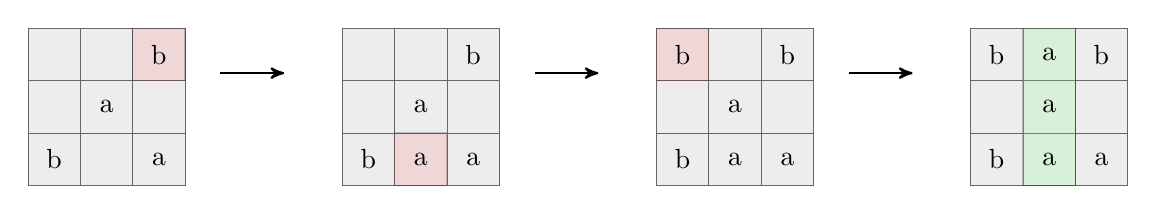
\begin{tikzpicture}[scale=0.95]
\newcommand\x{0}
\draw[step=0.7cm,draw=black!60,very thin,
fill=black!7] (\x+0,0) grid (\x+2.1,2.1) rectangle (\x+0,0);
\filldraw[fill=red!50!, draw=black, opacity=0.2] (\x+1.4,2.1) rectangle ((\x+2.1,1.4);
\draw[thick] (\x+0.35,0.35) node{b};
\draw[thick] (\x+1.75,1.75) node{b};
\draw[thick] (\x+1.05,1.05) node{a};
\draw[thick] (\x+1.75,0.35) node{a};
\draw[pil] (\x+2.5,1.5) -- node [above, text width = 3cm, align=center] {} (\x+3.5,1.5);

\newcommand\xx{4.2}
\draw[step=0.7cm,draw=black!60,very thin,
fill=black!7] (\xx+0,0) grid (\xx+2.1,2.1) rectangle (\xx+0,0);
\filldraw[fill=red!50!, draw=black, opacity=0.2] (\xx+.7,0.7) rectangle ((\xx+1.4,0);
\draw[thick] (\xx+0.35,0.35) node{b};
\draw[thick] (\xx+1.75,1.75) node{b};
\draw[thick] (\xx+1.05,1.05) node{a};
\draw[thick] (\xx+1.75,0.35) node{a};

\draw[thick] (\xx+1.05,0.35) node{a};
\draw[pil] (\xx+2.5,1.5) -- node [above, text width = 3cm, align=center] {} (\xx+3.5,1.5);

\newcommand\xxx{8.4}
\draw[step=0.7cm,draw=black!60,very thin,
fill=black!7] (\xxx+0,0) grid (\xxx+2.1,2.1) rectangle (\xxx+0,0);
\filldraw[fill=red!50!, draw=black, opacity=0.2] (\xxx+0,2.1) rectangle ((\xxx+0.7,1.4);

\draw[thick] (\xxx+0.35,0.35) node{b};
\draw[thick] (\xxx+1.75,1.75) node{b};
\draw[thick] (\xxx+1.05,1.05) node{a};
\draw[thick] (\xxx+1.75,0.35) node{a};
\draw[thick] (\xxx+1.05,0.35) node{a};
\draw[thick] (\xxx+0.35,1.75) node{b};

\draw[pil] (\xxx+2.5,1.5) -- node [above, text width = 3cm, align=center] {} (\xxx+3.5,1.5);

\newcommand\xxxx{12.6}
\draw[step=0.7cm,draw=black!60,very thin,
fill=black!7] (\xxxx+0,0) grid (\xxxx+2.1,2.1) rectangle (\xxxx+0,0);
\filldraw[fill=green!50!, draw=black, opacity=0.2] (\xxxx+0.7,0) rectangle ((\xxxx+1.4,2.1);

\draw[thick] (\xxxx+0.35,0.35) node{b};
\draw[thick] (\xxxx+1.75,1.75) node{b};
\draw[thick] (\xxxx+1.05,1.05) node{a};
\draw[thick] (\xxxx+1.75,0.35) node{a};
\draw[thick] (\xxxx+1.05,0.35) node{a};
\draw[thick] (\xxxx+0.35,1.75) node{b};
\draw[thick] (\xxxx+1.05,1.75) node{a};


\end{tikzpicture}
\caption{Sample game of (3,3,3) \textit{Tic-Tac-Toe} where player A wins by placing 3 consecutive objects a column; green indicates the winning column and red indicates the move made.} 
\label{nim_sample}
\end{figure}



\subsection{Game Description Language (GDL)}

Game Description Language (GDL), is a declarative logic programming language \citep{genesereth2005general}. It has been developed as a high-level knowledge representation formalism for axiomatising the rules of any game. Since our project attempts to model different games using a common framework, we use the formalizations of GDL to provide a uniform means of describing these games. There are ten game-independent relation constants defined in GDL, the ones with a special interest for us are the following.
\begin{itemize}
    \item \textit{role(a)} means that a is a role in the game.
    \item \textit{true(p)} means that the proposition p is true in the current state.
    \item \textit{does(r,a)} means that player r performs action a in the current state.
    \item \textit{next(p)} means that the proposition p is true in the next state.
    \item \textit{legal(r,a)} means it is legal for role r to play action a in the current state.
    \item \textit{goal(r,n)} means that player the current state has utility n for player r.
    \item \textit{terminal} means that the current state is a terminal state.    
\end{itemize}

\subsection{Answer Set Programming (ASP)}

According to \citet{lifschitz2019answer}:

\begin{displayquote}
``Answer set programming (ASP) is a form of declarative programming oriented towards difficult, primarily NP-hard, search problems."
\end{displayquote}

\justify
Answer Set Programming emerged in the early 1990s as a new declarative programming paradigm \citep{Gelfond1991}. It is based in nonmonotonic reasoning, deductive databases and logic programming with negation as failure. Since then, it has been considered a primary candidate as an effective knowledge representation tool. 

For the scope of this project, we use the \textit{clingo} ASP system, which is a combination of the grounder \textit{gringo} and the solver \textit{clasp}, developed by the Potassco research group from the University of Potsdam \citep{gebser2014clingo}. This system provides a useful API for \textit{python} which allows us to integrate our different approaches. 



\subsection{Inductive Learning of Answer Set Programs (ILASP)}

According to \citet{ILASP_system}:

\begin{displayquote}
``The goal of Inductive Logic Programming (ILP) is to find a hypothesis that explains a set of examples in the context of some pre-existing background knowledge."
\end{displayquote}

\justify


Inductive Logic Programming can be used in many applications. In the context of learning how to play games, the hypotheses we want to learn will correspond to the strategy. The background knowledge will be the rules of the game and the set of observations are the most desirable behavior in a given context. One of the advantages from using ILP over statistical machine learning approaches is that the learned hypotheses can be easily expressed in plain English and explained to a human user.

In this project, we use the Inductive Learning of Answer Set Programs (ILASP) framework, which is an inductive logic programming framework developed largely by Mark Law from the Imperial College London. It uses the system \textit{clingo} to generate answer sets explaining the examples. The framework can also generate \textit{weak constraints} as hypotheses using \textit{ordered examples} \citep{ILASP_system}. This particular feature allows us to find a game strategy in the form of weak constraints given an ordered set of preferred moves in a given context. Such characteristics make it a great fit to learn strategies for games defined in ASP.


\begin{figure}[H]
\centering
\fbox{
\includegraphics[trim={1.5cm 0.5cm 0.4cm 0.1cm},clip,width=\linewidth]{example_ilasp_1.png}
}
\caption{Sample ILASP program; excerpt from ILASP v3.1.0 manual in \citet{law2017inductive}} 
\end{figure}

\subsubsection{Definitions and Syntaxes}

\begin{description}
    \item [Weak constraint] \hfill \\
    A weak constraint represents an expression of preference in ASP; such that resulting answer sets of a program $P$ can be ranked by preference. Therefore, a weak constraint represents a form of optimization in ASP.
    \item [Partial interpretation] \hfill \\
    A partial interpretation $E$ is a pair of sets of atoms $E^{inc}$ and $E^{exc}$, called the inclusions and exclusions of $E$. We write $E$ as $\langle E^{inc},E^{exc} \rangle$. An answer set $A$ is said to extend $E$ if it contains all of the inclusions ($E^{inc} \subseteq A$) and none of the exclusions ($E^{exc} \cap A = \emptyset$).
    \item [Positive/Negative example] \hfill \\ A positive/negative example is a partial interpretation and can be specified in ILASP as
    \texttt{$\#$pos(example$\_$name,$\left\{e_1^{inc},\ldots,e_m^{inc}\right\},\left\{e_1^{exc},\ldots,e_n^{exc}\right\}$)} or \\
    \texttt{$\#$neg(example$\_$name,$\left\{e_1^{inc},\ldots,e_m^{inc}\right\},\left\{e_1^{exc},\ldots,e_n^{exc}\right\}$)} respectively, \\where \texttt{example$\_$name} is a unique identifier for the example.
    \item [Language bias] \hfill \\
    A language bias in ILASP refers to the search space of possible hypotheses in which inductive solutions should be searched for. These are typically encoded by mode declarations. An example of this is \texttt{$\#$modeo}, which expresses what is allowed to appear in the body of a learned weak constraint.
    \item [Ordering example] \hfill \\ An ordering example is a tuple $o = \langle e_1,e_2 \rangle$, where $e_1$ and $e_2$ are partial (positive-example) interpretations.
    \item [Brave ordering\footnotemark] \hfill \\
    An ASP program $P$ bravely respects $o$ iff $\exists A_1,A_2 \in AS(P)$, such that $AS(P)$ is the answer set of $P$, $A_1$ extends $e_1$, $A_2$ extends $e_2$ and $A_1 \succ_p A_2$.
    \item [Cautious ordering\text{\footnotemark[\value{footnote}]}] \hfill \\
    An ASP program $P$ cautiously respects $o$ iff $\forall A_1,A_2 \in AS(P)$, such that $AS(P)$ is the answer set of $P$, $A_1$ extends $e_1$, $A_2$ extends $e_2$ and $A_1 \succ_p A_2$.
\end{description}

\footnotetext{
\textbf{Note:} Given two positive examples $e_1$ and $e_2$ with identifiers \texttt{id}$_1$ and \texttt{id}$_2$, the ordering example $\langle e_1,e_2 \rangle$ can be expressed in ILASP as \texttt{$\#$brave$\_$ordering(order$\_$name,id$_1$,id$_2$)} or
\texttt{$\#$cautious$\_$ordering(order$\_$name,id$_1$,id$_2$)}, where \texttt{order$\_$name} is an optional identifier for the ordering example.
}

\subsubsection{ILASP Framework}

\justify
\citet{law2017inductive} provides a succinct overview of the ILASP framework to inductively learn hypotheses from answer sets:

\begin{displayquote}
Given an ASP program $B$ called the background knowledge, a set of ASP rules $S$ called the search space and two sets of partial interpretations $E^{+}$ and $E^-$ called the positive and negative examples respectively, the goal is to find another program $H$ called a hypothesis such that:
\begin{enumerate}
    \item $H$ is composed of the rules in $S$ ($H \subseteq S$)
    \item Each positive example is extended by at least one answer set of $B \cup H$ (can be a different answer set for each positive example)
    \item No negative example is extended by any answer set of $B \cup H$
\end{enumerate}
\end{displayquote}

\justify
Similarly, \citet{law2017inductive} provides a framework for extending the above-mentioned method to learn weak constraints from positive examples and ordered answer sets. For brevity, we will exclude the full details of this process; but it is similar to the learning process defined above. For the scope of this project, we will use ordering examples to inductively learn weak constraints. As a result, we will only consider positive examples as partial interpretations.


\subsection{Game Tree}

In order to learn any game strategies, we would first have to conceptualize the concept of a two-player game in a logical and well-computable format. One such useful format would be a game tree. A game tree is a directed graph whose nodes are states of the game and whose edges are action.
% Such that for every node has as many children as legal actions.
The \textit{complete game tree} of a game starts at the initial position and contains all legal actions from each position. 

For this project, we represent such trees using the \texttt{anytree} Python package, which is publicly available in the Python Package Index (PyPI) repository. Given a game tree $T$, we assume the following conventions pertaining to tree objects in the scope of this paper:

\begin{enumerate}
    \item $T(i,j,p,d)$ refers to the node with identifier $j$ present at depth $d$ whose parent node has identifier $i$ at depth $d-1$, where player $p$ is playing the current round.
    \item For cases where no parent node exists, such as for the root node, the following convention will be used: $T(\text{null},j,p,d)$
    \item $i$, $j$ and $d$ defined above all exist in $\mathbb{N}_0$
    \item $d$ has an upper bound of $D$, where $D$ refers to the maximum depth of tree $T$. $d$ corresponding to $0$ would imply the root node.
    \item We will assume that only two players play the corresponding games alternately. As a convention, we will define these players as player $a$ and player $b$. Therefore, $p$ can take the values of $a$ or $b$.
    \item $T(i,j,p,d)[s]$ will refer to the state $s$ of the node $T(i,j,p,d)$. This state contains information on the current configuration of the game and whether the state is terminal. 
    \item $T(i,j,p,d)[a]$ will refer to the action $a$ that was taken to reach the node $T(i,j,p,d)$. Only the root node will have no associated action.
    \item $T(i,j,p,d)[v]$ will refer to the reward value of the node $T(i,j,p,d)$. This will usually only be defined for terminal nodes of a game tree.
    \item $\mathcal{M}(s_0,a_0,\cdots,a_n-1,s_n)$ will refer to a match in the game as a sequence of states. A match can be obtained form a path starting in root node and traversing the tree util a leaf node is reached.
    \item Given a match $\mathcal{M}_a(s_0,a_0,\cdots,a_n-1,s_n)$ we can generate a tree $T_a$ with a single branch rooted in state $s_0$.
    % \item We will work only with \textit{zero-sum games}. This implies that the sum of all rewards is equal to the sum of all losses. Hence, if player $a$ receives a positive reward of $+1$ then player $b$ receives a negative reward of $-1$.
\end{enumerate}

\begin{figure}[H]
    \centering
    \includegraphics[width=0.85\linewidth]{tree.png}
    \caption{Complete game tree for Nim with initial configuration (3,1,0,0). The actions are represented as part of the nodes instead of the edges.}
\end{figure}

\section{Methodologies}
\label{methods}
\subsection{Game simulation}

To simulate the entirety of a game, we utilized a combined ASP and Python framework, which is summarized in a later subsection. In regards to ASP, we created an encoding, namely \texttt{background.lp}, representing the dynamics of the game to perform a single time step. This encoding depends on a set of facts defining the current state of the game. For the initial state, such facts are saved in a file and for the following states, they are computed throughout the simulation. Initial states are saved in files \texttt{*initial.lp}, where * implies a prefix. Both sets of encodings are written using the GDL formalisms, such that the same variable and atom naming conventions can be used across all games. For the game of Nim illustrated in Figure 4, the background program and initial state can be found in Figure 5 and Figure 6, respectively. 

\lstset
{ %Formatting for code in the appendix
    language=Prolog,
    basicstyle=\footnotesize,
    numbers=left,
    stepnumber=1,
    showstringspaces=false,
    tabsize=1,
    breaklines=true,
    breakatwhitespace=false,
    frame=single,
    xleftmargin=2em
}

\begin{center}
    \begin{lstlisting}[] 
#const max_removable = 6. 
#const max_sticks = 7. 
#const num_piles = 4.

% Roles
role(a). role(b).

% Base (All possible values inside 'true')
base(has(P,M)):- P=1..num_piles,M=0..max_sticks.
base(control(X)) :- role(X).

% Input (All possible actions)
input(X,remove(P,N)) :- P=1..num_piles, 
                        N=1..max_removable,
                        role(X).

% Legal actions
legal(X,remove(P,N)) :- true(has(P,M)), 
                        P = #min{L:true(has(L,M))},
                        N=1..max_removable, N<=M, 
                        true(control(X)), 
                        not terminal.

% Action selection
0 {does(X,A)} 1 :- legal(X,A), not terminal.
:- does(X,Y), does(X,Z), Y < Z.
:- not does(X,_), true(control(X)), not terminal.

% State transition
next(control(b)) :- true(control(a)), not terminal.
next(control(a)) :- true(control(b)), not terminal.
next(has(P,N-M)) :- does(_,remove(P,M)), 
                    true(has(P,N)), not terminal.
next(has(P,N)) :- not does(_,remove(P,_)), 
                  true(has(P,N)), not terminal.

% Goals
goal(X,-1) :- #sum{N,M:true(has(M,N))}=0, true(control(X)).
goal(X,-1*G):- goal(Y,G), role(X), X!=Y.

% Terminal state
terminal :- goal(_,_).
    \end{lstlisting}
    \captionof{figure}{\texttt{background.lp} encoding for dynamics of the game of Nim}
\end{center}

\begin{center}
    \begin{lstlisting}[] 
true(has(1,3)).
true(has(2,1)).
true(has(3,0)).
true(has(4,0)).
true(control(a)).
    \end{lstlisting}
    \captionof{figure}{ASP encoding the initial state of Figure 4}
\end{center}

Throughout the game simulation, each node $T(i,j,p,d)$ of the tree can expanded with the following actions. Using the background program $P$ and the set of facts representing the state $T(i,j,p,d)[s]$, we call \textit{clingo} in search for the next possible states. This call will obtain one answer set per legal action. For each answer set, we proceed to create a new children node $T(i,j',p',d+1)$ were its state $T(i,j',p',d+1)[s]$ is constructed by replacing $\texttt{next/1}$ with predicate $\texttt{true/1}$. To exemplify such process, show the output when we call \textit{clingo} with the encodings from Figure 5 and Figure 6. This call will return 4 answer sets corresponding to the first level of the tree in Figure 4.

\begin{figure}[H]
\centering
\begin{varwidth}{\linewidth}
\begin{verbatim}
Answer: 1
next(has(3,0)) next(has(4,0)) next(control(b))
does(a,remove(2,1)) next(has(1,3)) next(has(2,0))

Answer: 2
next(has(3,0)) next(has(4,0)) next(control(b)) 
does(a,remove(1,2)) next(has(2,1)) next(has(1,1))

Answer: 3
next(has(3,0)) next(has(4,0)) next(control(b)) 
does(a,remove(1,3)) next(has(2,1)) next(has(1,0))

Answer: 4
next(has(3,0)) next(has(4,0)) next(control(b)) 
does(a,remove(1,1) next(has(2,1)) next(has(1,2))
\end{verbatim}
\end{varwidth}
\end{figure}

Using the Python Application Programming Interface (API) for \textit{clingo}, we can then extrapolate this process to simulate multiple time steps in the game and construct the game tree. Further, when given a strategy in the form of weak constraints, such encoding can be included, enforcing an order over the answer sets. Such ordering will allow the player you select the best action (answer set) according to the optimization defined by the weak constraints.


\subsection{Learning Approaches}

\subsubsection{Minimax Algorithm}

The minimax algorithm is a recursive tree-search algorithm which has its origins in combinatorial game theory for choosing the next best move of a two-person zero-sum game. The intuition behind this algorithm lays in the fact that every movement made by player $a$ will aim to maximize the reward of $a$, while player $b$ will try to minimize this same reward. This algorithm will first construct the complete game tree $T$ of depth $D$ for alternately-playing players $p$ and $p'$. All the terminal nodes of the tree will be annotated with reward values $v$ extracted from predicate $\texttt{goal/1}$. Then, it will proceed to compute the minimax score $M$ of any node on the tree starting on the leaves by utilizing the following piecewise function:

\begin{equation}
M(j,p,d-1) = 
\begin{cases} 
\underset{k}{\max} ~ T(j,k,p',d)[v], & p = a\\[10pt]
\underset{k}{\min} ~ T(j,k,p',d)[v], & p = b\\[10pt]
\end{cases}
\end{equation}

\justify
where:
\begin{flalign*}
~~~ &d = \text{depth of node on the decision tree: } d \in [0,D], ~ d \in \mathbb{N}_0& \\
~~~ &j = \text{$j$'th parent node on depth $d-1$ where $M$ is to be evaluated: } j \in \mathbb{N}_0& \\
~~~ &k = \text{$k$'th child node of parent node $j$ on depth $d$ where $v$ is defined: } k \in \mathbb{N}_0& \\
%~~~ &M(i,p,D) = T(i,p,D)[v]\text{: minimax values at leaves are equal to reward values}& \\
~~~ &p, p' = \text{unique player playing on specified depth:} ~ p,p' \in {\cal P} = \left\{a,b\right\},~ p' = {\cal P} \setminus p &\\
~~~ &\textbf{Note: } \text{We assume the positive reward player $a$ maximizes $M$ while the}& \\
~~~ &\text{negative reward player $b$ minimizes $M$} &
\end{flalign*}

\justify
Given the piecewise function $M$ defined above, we present below the pseudocode used for the minimax algorithm in our project. The time complexity of this algorithm is $O(b^D)$, while the space complexity is $O(bD)$; where $b$ is the average branching factor and $D$ is the maximum depth of the game tree \citep{russell2016artificial}.

\begin{algorithm}
  \caption{Minimax}
  \begin{algorithmic}[1]
  \Require{Game tree $T$ of depth $D$ with reward values $v$ at terminal nodes}
  \Ensure{Game tree $T'$ with minimax values at all nodes}
  \Statex
    \Function{Minimax}{$T$}
      \State $T' \gets T$ \Comment{Make local copy of $T$ as $T'$}
      \For{$d \gets D-1$ to $0$} \Comment{Loop upwards from bottom of $T'$}
      \ForEach{node $T(i,j,p,d)$} \Comment{Loop each node at depth $d$}
        \State $T'(i,j,p,d)[v] \gets M(j,p,d)$ \Comment{Update $T'$ with $M$}
      \EndFor
      \EndFor
      \State \textbf{return} $T'$ \Comment{Return updated game tree $T'$}
    \EndFunction
  \end{algorithmic}
\end{algorithm}

\begin{figure}[H]
  \centering
  \includegraphics[width=0.9\linewidth]{tree-minmax.png}
  \caption{Tree resulting from applying the Mimimax algorithm to the complete tree in Figure 4. Green nodes have a positive score, implying a winning strategy for player $a$, while red nodes represent an position where player $b$ will win.}
\end{figure}

In the example given on Figure 7, all nodes are scored using the minimax function $M$, defined in formula 1. Since the score of the root node is $1$, player $a$ can assure a winning outcome by following the path down the tree choosing the nodes that have this score, such nodes are marked in green. We can notice this path is the same one as the one defined on Figure 1.

\subsubsection{Pruned Minimax Algorithm}

The Minimax algorithm has many variants that aim to make it more efficient by decreasing the number of nodes that are evaluated. One of the best-known algorithms, called Alpha–beta pruning \citep{knuth1975analysis}, stops evaluating a move when at least one possibility has been found that proves the move to be worse than a previously examined move. Our proposed Pruned Minimax algorithm is based on this idea while including the optimization statements existent in \textit{clingo}. The construction is performed similarly to the Depth-first search (DFS) algorithm for traversing or searching tree. 

\vspace{10px}
\textbf{Explicit time encoding}\\

In GDL we use predicate \texttt{true(F)} to indicate that \texttt{F} holds in the current state and \texttt{next(F)} when it holds in the next state. This syntax can be translated to a single predicate \texttt{holds(F,T)} where the time step in which \texttt{F} holds is specified with \texttt{T}. This notation is used for planning problems and it is based on event calculus \cite{shanahan1999event}. 
With the new encoding, each stable model will represent a full match containing the actions performed in each time step.
This representation makes use of all the advantages provided by \textit{clingo} for planning problems such as incremental solving. In order to translate our current encoding to this new format we need to perform the following steps:
\begin{enumerate}
\item Replace \texttt{true(F)} by \texttt{holds(F,T)}
\item Replace \texttt{next(F)} by \texttt{holds(F,T+1)}
\item Replace \texttt{p(F1..Fn)} by \texttt{p(F1..Fn,T)} where $p\in \{ legal,does,goal,terminal\}$
\item In every rule where a replacement was made, add the time in in the body with predicate \texttt{time(T)}.
\item Add a new fact with all possible time steps \texttt{time(0..N)} using a predefined horizon $N$.
\end{enumerate}


\vspace{10px}
\textbf{Optimization}\\

The system \textit{clingo} comes with a set of optimization statements that enforce an order in the answer sets. With the optimization statement \\ 
\texttt{\#maximize\{N,T:goal(a,N,T)\}} 
we can find the stable model which maximizes the reward $N$ given to player $a$ defined in the predicate \texttt{goal(a,N,T)}, 
were $T$ is the time step in which the goal was reached. By adding this to the explicit time encoding of a game, we will find the match that maximizes the reward for $a$. 
However, this optimization assumes that player $b$ will make the moves that generate the best outcome for his opponent. 
We will call this match $\mathcal{M}_a$ an optimized match for $a$. 
To select actions for player $b$ working on his own benefit, we would need to minimize the reward of $a$ in the time steps where player $b$ has control. 
Minimizing the reward of $a$ can be achieved with the optimization statement 
\texttt{\#minimize\{N,T:goal(a,N,T)\}.} Sadly, the alternation of different optimizations in every time step is not allowed in \textit{clingo}. Nonetheless, we can perform such alternation with multiple calls to the solver in a clever manner as it is described bellow. 

\vspace{10px}
\textbf{The algorithm}\\

The algorithm in this approach uses the defined explicit time encoding to find optimal matches (stable models) and proceeds to modify the matches such that they are optimizing both players. This process, which we will call \textit{validation}, will construct a scored-pruned game tree leaving irrelevant parts of the tree unexplored. The pseudocode for the algorithm can be found below in Algorithm 2 and 3. The recursive function \textit{validate} will perform a bottom-up validation from the the end of the match up until step $i$. Lines 3 and 4 make sure that the rest of the match is fixed and a new part is explored by negating the action already taken at each step. Lines 14 and 15 append new paths to the game tree. The pruning is performed on lines 19 and 21 where the current branch of the tree remains only explored by the clingo call (Line 7 or 9). Validation of this branch unnecessary since the current result can't be improved\footnote{These unexplored branches can be found in Figure 8 with blank nodes.}. The recursive call in line 23 will proceed to explore the required parts of the tree by validating the match. Finally, the case on line 29 will update the match and the score of the node with an improved action for the player in turn. 


\begin{algorithm}
  \caption{Pruned minimax}
  \begin{algorithmic}[1]
  \Require{The explicit encoding $P_e$ and the initial state of the game}
  \Ensure{A tree $T$ for the pruned tree}
  \Statex
    \Function{PrunedMinimax}{$P_e$,$s_0$}
      \State $\mathcal{M}_a(s_0,a_0,\cdots,a{n-1}, s_n) \gets clingo(P_e,s_0)$ \Comment{Compute $\mathcal{M}_a$}
      \State $T \gets [s_0,\cdot,s_n]$ 
      \Comment{Create a tree with only the branch from $\mathcal{M}_a$} 
      \State $M_v \gets validate(M_a,0)$
    \EndFunction
  \end{algorithmic}
\end{algorithm}

\begin{algorithm}
  \caption{Validate match}
  \begin{algorithmic}[1]
    \Require{An optimized match $M_v$ to be validated from a time step $i$}
    \Ensure{A validated match where both players play to their advantage}

    \Statex
      \Function{validate}{$\mathcal{M}_v(s_0,a_0,\cdots,s_i,a_i,\cdots,s_n)$,$i$}
        \For{$k \gets n-1$ to $i$} \Comment{Loop upwards each state untill $s_i$}
          \State $P_k \gets [s_0,a_0,\cdots,s_k]$ \Comment{\small Fix states and actions untill $k$}
          \State $P_k \cup not\; a_k$ \Comment{\small Negate action $a_k$ to explore other possible actions}
          \State{$p_c \gets $ player in control on $s_k$ }
          \If{$a == p_c$}
          \State {$M_{p_c} \gets clingo(P_e,P_k,max)$} 
          \Comment{Compute match from $k$ maximizing $a$}
          \Else \State{$M_{p_c} \gets clingo(P_e,P_k,min)$}
          \Comment{Compute match from $k$ minimizing $a$}
          \EndIf
          \If{$M_{p_c}$ is $None$} \Comment{No other possible action than $a_k$} \State{\textbf{continue}} \Comment{Go to next k}
          \EndIf
          % \State{$n_{k-1} \gets $ parent node of $s_k$ from $T$ }

          \State{$T_{p_c} \gets [s_{p_c}k+1,\cdots,s_{p_c}m]$}
          \Comment{Create a tree with only the branch from $M_{p_c}$}
          \State{Hang unexplored branch $T_{p_c}$ from the parent of $s_k$ in $T$}

          \State{$r_o \gets M_{p_c}[p_c]$} \Comment{Reward for $p_c$ in optimized}
          \State{$r_v \gets M_{v}[p_c]$} \Comment{Reward for $p_c$ in old match}
          
          \If{$r_v>r_o$} 
          \Comment{$a_k$ is the best action for $p_c$}
          \State{
            $T(x,s_k,k,p_c)[v] \gets r_v$}
          
          \ElsIf{$r_v==r_o$}  
          \Comment{$a_k$ is as good as the best outcome for $p_c$}
          \State{$T(x,s_k,k,p_c)[v] \gets r_v$}

          \ElsIf{$r_v<r_o$}  
          \Comment{Action in $M_{p_c}$ potentially better than $a_k$ for $p_c$}
          \State{$M_{p_cv} \gets validate(M_{p_c},k+1)$}
          \Comment{Validates the match and explores $T_{p_c}$}
          \State{$r_{p_cv} \gets M_{p_cv}[p_c]$} \Comment{Reward for $p_c$ in validated match}
            \If{$r_v>r_{p_cv}$} 
            \Comment{$a_k$ is the best action for $p_c$}
            \State{$T(x,s_k,k,p_c)[v] \gets r_v$}
            
            \ElsIf{$r_v==r_{p_cv}$}  
            \Comment{$a_k$ is as good as the best outcome for $p_c$}
            \State{$T(x,s_k,k,p_c)[v] \gets r_v$}

            \ElsIf{$r_v<r_{p_cv}$}  
            \Comment{The action in $M_{p_cv}$ is better for $p_c$}
            \State{$M_v \gets M_{p_cv}$} 
            \State{$T(x,s_k,k,p_c)[v] \gets r_{p_cv}$}
            \EndIf 
          \EndIf 
        \EndFor
        \State \textbf{return} $M_v$ \Comment{Return match $M_v$ validted from step $i$}
      \EndFunction
        
    \end{algorithmic}
\end{algorithm}

\begin{figure}[H]
\centering
  \includegraphics[width=0.9\linewidth]{tree-pruned.png}
  \caption{Tree resulting from applying the Pruned Minimax algorithm to the complete tree in Figure4. White branches are those that remain only explored by clingo but never validated.}
\end{figure}

\vspace{10px}
\textbf{Learning ASP rules}\\

During the validation process, there are some key points where we become aware of one action being better than another. This points are on lines 18, 25 and 29 of Algorithm 2 where a player should take a specific action to achieve a better reward. It is in these sections where we can generate rules that define a strategy or other type of data as explained in the next subsection. This strategy can be considered an abstract representation of the scored game tree. Within the Algorithm 2 we can easily use the current information to generate rules of the form:

\vspace{30px}

\begin{minipage}{0.90\textwidth}
  \vspace{5px}
  \begin{verbatim}
best_do(a,remove(2,2),T):-  holds(control(a),T),
                            holds(has(1,0),T), 
                            holds(has(2,2),T),
                            holds(has(3,0),T),
                            holds(has(4,0),T).
  \end{verbatim}
  \hfill
\end{minipage}
\begin{minipage}{0.05\textwidth}
  \hfill (2)
  \vspace{30px}
\end{minipage}

These rules will define under which state context, described by predicate \texttt{holds/2} is it better to perform a certain action. In this case, for the game on Nim we are stating that: In a state where player $a$ has control and only pile $2$ has $2$ counters it would be best to remove from pile $2$ both counters. 

It is important to notice that the rules in this approach will only be correct when the body defines one unique state of the game. This will imply a new requirement that must be fulfilled by the background encoding for this approach to be correct.

In order to enforce the use of these preferred actions as an strategy all we need to do is add the following rule to the strategy.

\vspace{30px}

\begin{minipage}{0.90\textwidth}
  \vspace{5px}
  \begin{verbatim}
1{does(P,A,T):best_do(P,A,T)}1:- time(T),
                                 not goal(_,_,T),
                                 {best_do(P,A,T)}>0,
                                 true(control(P)).
  \end{verbatim}
  \hfill
\end{minipage}
\begin{minipage}{0.05\textwidth}
  \hfill (3)
  \vspace{30px}
\end{minipage}


A desirable characteristic of a strategy is to be generalizable. Since the generated rules use constants, this can't be achieved. However, given a formalization allowing us to decide whether a term should be converted into a variable or not, we can substitute each some constants by variables. For this formalization we used a function $f:P,i \to Bool$ where every function name in $P$ has an associated boolean value for each attribute position $i$ indicating if it should be transformed into a variable. We will also need additional literals to ensure different variables are not substituted by the same constant during grounding. The following rule would correspond to the previous example generalized with variables using only $f(has,0)$,$f(control,0) $ and $f(best\_do,0)$ are assigned to true. 


\vspace{30px}

\begin{minipage}{0.90\textwidth}
  \vspace{5px}
  \begin{verbatim}
best_do(Va,remove(V2,1),T):-  holds(control(Va),T),
                              holds(has(V1,0),T), 
                              holds(has(V2,2),T),
                              holds(has(V3,0),T),
                              holds(has(V4,0),T),
                              V1!=V3,V1!=V2,V1!=Va,
                              V3!=V2,V3!=Va,V2!=Va.
    \end{verbatim}
  \hfill
\end{minipage}
\begin{minipage}{0.05\textwidth}
  \hfill (4)
  \vspace{30px}
\end{minipage}


With this generalize rule we can apply the strategy to any permutation over the piles and players. Further, by applying these rules during the construction of the tree we can prune more branches with the learned information. This is exemplified in figures 9 and 10. In Figure 10 we can notice how the right branch of the tree is never explored. This is because during the construction of the left branch in the bottom left corner we learned the rule mentioned above. When this rule is generalized it becomes applicable for player $b$. Since player $b$ now knows that removing two counters is better, the green section of the right branch from Figure 9 is removed leaving the only possible outcome of -1 and becoming unnecessary to be further explored by $a$.


\begin{minipage}{0.45\textwidth}
  \centering
  \vspace{10px}
  \includegraphics[height=1.3\textwidth]{tree-norules.png}
  \captionof{figure}{Pruned minimax tree without applying learned rules.}
  \vspace{15px}

\end{minipage}
\begin{minipage}{0.45\textwidth}
  \centering
  \vspace{10px}
  \includegraphics[height=1.3\textwidth]{tree-rules.png}
  \captionof{figure}{Pruned minimax tree applying learned rules.}
  \vspace{15px}

\end{minipage}


% \vspace{10px}
% \textbf{Generating ordered examples}\\

% The same decisive points mentioned above can also be used to generate ordered examples. 




\subsubsection{Weak Constraints from ILASP}

For this approach, our objective is to find more generalized strategies in the form of weak constraints using ILASP. Since we already have the background knowledge defined, we just need to define a set of ordered positive examples and a language bias. 

\vspace{10px}
\textbf{Generating ordered examples}\\

The decisive points mentioned in the previous section to learn rules can also be used to generate ordered examples. By running the Pruned Minimax algorithm we can construct examples with small modifications to the code. The ordered example corresponding to rule in Example 2 would be the following:

\begin{verbatim}
#pos(e0,{}, {}, {
    true(control(a)). true(has(1,0)). true(has(2,2)). 
    true(has(3,0)). true(has(3,0)). does(a,remove(2,2)). 
}).
#pos(e1,{}, {}, {
    true(control(a)). true(has(1,0)). true(has(2,2)). 
    true(has(3,0)). true(has(4,0)). does(a,remove(2,1)). 
}).

#brave_ordering(e0,e1).
\end{verbatim}

\textbf{Defining language bias}\\


Once we have the examples we only need to define a language bias. This process in most cases will require time to define how the strategy (Hypothesis) might look. The code in Figure 11 shows the language bias used for the game if TicTacToe. Line 1 to 4 define the possible atoms that might appear in the week constraint. These atoms include a cell being free, tree cells being on a line and the values for each cell. It is important to notice the use of \texttt{next/1} instead of \texttt{true/1}. Creating a strategy dependent on the next state will automatically include the effect of the action taken, thus indirectly ordering the actions. Lines 5 to 8 define the configuration for the possible weights, priorities and variables.


\begin{center}
  \begin{lstlisting}[] 
#modeo(3,next(has(var(player),var(cell))),(positive)).
#modeo(1,in_line(var(cell),var(cell),var(cell)),(positive)).
#modeo(1,next(free(var(cell))),(positive)).
#modeo(1,next(control(var(player))),(positive)).
#weight(-1).
#weight(1).
#maxp(2).
#maxv(4).
  \end{lstlisting}
  \captionof{figure}{Language bias for the game of TicTacToe}
\end{center}


For the game of Nim we wanted to find a strategy close to the mathematical one defined in \nameref{nim}. To do so, we first included in the encoding a set of facts for the binary representation of a number. Atom \texttt{binary(N,D,V)} can be read as number $N$ has the value $V\in\{1,0\}$ in position $D\in\{1,2,3\}$. Since the expected strategy is more complex and by using the existent predicates the search space is too big, we used the language bias for predicate invention. For the invention, ILASP will generate normal ASP rules in addition to the weak constraints. In the code on Figure 12, lines 5 to 7 define the invented predicates that will go in the head of the ASP rules where the body will be defined by lines 8 to 11. Lines 12 and 13 describe the possible predicates for the weak constraints.


\begin{center}
  \begin{lstlisting}[] 
#constant(pile,1).
#constant(pile,2).
#constant(pile,3).
#constant(pile,4).
#modeh(b(var(pile),var(d),var(bool)),(positive)).
#modeh(nim_sum(var(d),var(total)+var(bool),var(pile)),(positive)).
#modeh(nim_sum(var(d),0,0),(positive)).
#modeb(1,b(var(pile),var(d),var(bool)),(positive)).
#modeb(1,nim_sum(var(d),var(total),var(pile)-1),(positive)).
#modeb(1,binary(var(num),var(d),var(bool)),(positive)).
#modeb(1,next(has(var(pile),var(num))),(positive)).
#modeo(1,nim_sum(var(d),var(t),const(pile))).
#modeo(1,var(t)\2 != 0).
#weight(1).
#weight(-1).
#maxp(1).
#maxv(4).
  \end{lstlisting}
  \captionof{figure}{Language bias for the game of Nim}
\end{center}

As a final step, we will use the generated ordered examples, the language bias and the background encoding to call the ILASP framework. The call will return a hypothesis representing a strategy that will order the examples. If no Hypothesis is found the result will be UNSAT.

\newpage
\subsection{Workflow Summary}
\label{summary}
\vspace{-10pt}
\begin{figure}[H]
\centering
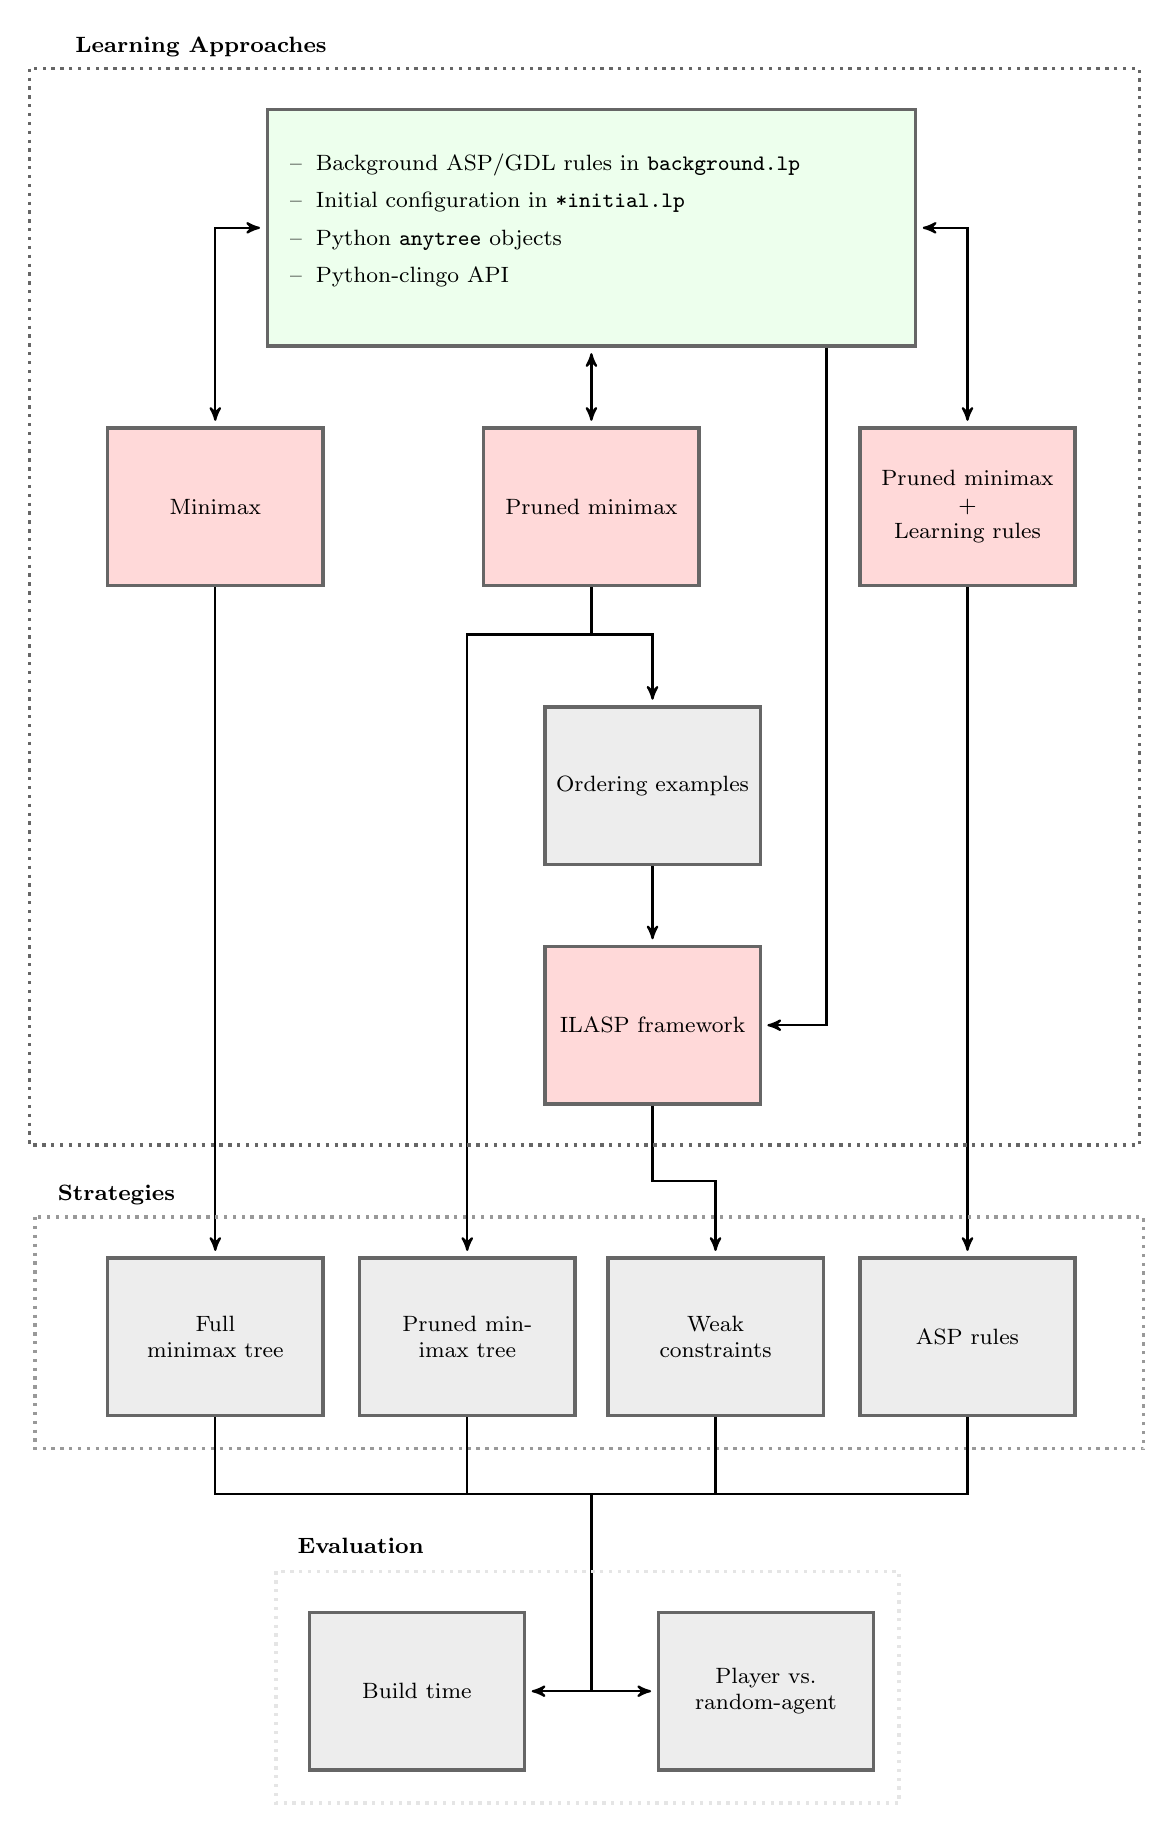
\begin{tikzpicture}[node distance=1cm,font=\footnotesize]
\node[vblock3, fill=green!07] (middleBig) {\vspace{-12pt} 
\begin{itemize}[leftmargin=0.5cm]
    \item[--] Background ASP/GDL rules in \texttt{background.lp}
    \item[--] Initial configuration in \texttt{*initial.lp}
    \item[--] Python \texttt{anytree} objects
    \item[--] Python-clingo API
\end{itemize}};
\node[recBlock2, below = of middleBig,fill=red!15] (prunedMinimax) {Pruned minimax};
\node[recBlock2, left = 2.0cm of prunedMinimax,fill=red!15] (basicMinimax) {Minimax};
\node[recBlock2, right = 2.0cm of prunedMinimax,fill=red!15] (combMinimax) {Pruned minimax \\ $+$ \\ Learning rules};
\node[recBlock2, below right = 1.5cm and -2cm of prunedMinimax] (orderedEgs) {Ordering examples};
\node[vblock4, below = 1cm of orderedEgs,fill=red!15] (ilasp) {ILASP framework};
\node (cross) at ($(prunedMinimax.south)+(0.0,-0.6)$) {};
\draw[<->,thick,shorten >=2pt,shorten <=2pt] (basicMinimax.north) |- (middleBig.west) {};
\draw[<->,thick,shorten >=2pt,shorten <=2pt] (prunedMinimax) -- (middleBig) {};
\draw[<->,thick,shorten >=2pt,shorten <=2pt] (combMinimax.north) |- (middleBig.east) {};
\draw[pil2] (cross.center) -| (orderedEgs.north) {};
\draw[thick] (prunedMinimax.south -| cross.north) -- (cross.center) {};
\node[recBlock2, below = 8.5cm of basicMinimax] (resBasicMinimax) {Full \\ minimax tree};
\node[recBlock2, below left = 8.5cm and -1.2cm of prunedMinimax] (resPrunedMinimax) {Pruned minimax tree};
\node[recBlock2, below right = 8.5cm and -1.2cm of prunedMinimax] (resILASP) {Weak \\constraints};
\node[recBlock2, below = 8.5cm of combMinimax] (resComb) {ASP rules};
\draw[pil2] (basicMinimax) -- (resBasicMinimax) {};
\draw[pil2] (combMinimax) -- (resComb) {};
\draw[pil2] (orderedEgs) -- (ilasp) {};
%\draw[pil] (ilasp.south) -- (resILASP.north -| ilasp.south) {};
\draw[pil2] (ilasp.south) |- ($(ilasp)!0.5!(resILASP)$) -| (resILASP.north) {};
\draw[pil2] (cross.center) -| (resPrunedMinimax) {};
\draw[pil2] (middleBig.-27) |- (ilasp.east) {};
\draw[black!60,very thick,dotted] ($(middleBig.north west)+(-3.0,0.5)$) rectangle ($(ilasp.south east)+(4.8,-0.5)$);
\draw[black!40,very thick,dotted] ($(resBasicMinimax.north west)+(-0.9,0.5)$) rectangle ($(resComb.south east)+(0.85,-0.4)$);
\node (cross2) at ($(resPrunedMinimax)!0.5!(resILASP)+(0.0,-2.0)$) {};
\draw[thick] (resBasicMinimax) |- (cross2.center) {};
\draw[thick] (resComb) |- (cross2.center) {};
\draw[thick] (resPrunedMinimax.south) -- (cross2.center -| resPrunedMinimax.south) {};
\draw[thick] (resILASP.south) -- (cross2.center -| resILASP.south) {};
\node[recBlock2] at ($(resPrunedMinimax)!0.2!(resBasicMinimax)+(0.0,-4.5)$) (build) {Build time};
\node[recBlock2] at ($(resILASP)!0.2!(resComb)+(0.0,-4.5)$) (pvp) {Player vs. random-agent};
\draw[thick,->,thick,shorten >=2pt] (cross2.center) |- (build) {};
\draw[thick,->,thick,shorten >=2pt] (cross2.center) |- (pvp) {};
\draw[black!10,very thick,dotted] ($(build.north west)+(-0.4,0.5)$) rectangle ($(pvp.south east)+(0.3,-0.4)$);
\node [left=of middleBig,yshift=2.3cm,xshift=1.9cm] {\textbf{Learning Approaches}};
\node [left=of resBasicMinimax,yshift=1.8cm,xshift=2.0cm] {\textbf{Strategies}}; 
\node [left=of build,yshift=1.85cm,xshift=2.6cm] {\textbf{Evaluation}}; 
\end{tikzpicture}
\caption{Summary of workflow/methodologies in this project separated into three different categories; namely learning approaches, strategies and evaluation}
\end{figure}

% todo: update information based on changes in previous sections
% possible: consider parallel arrows instead of superimposed

\section{Results}
\label{results}

We divided the evaluation into two phases. In the first one, we examined the process of learning each strategy and the results. For the second one, we tested their performance during gameplay. The presented results ran on a 2.6 GHz Quad-Core Intel Core i7 processor under MacOs. The benchmarks were performed using three different initial configurations for each game of increasing complexity, namely, \textit{Small(S), Medium(M)} and \textit{Large(L)}. These divisions were designed to provide information about the scalability of each approach into the \textit{Classical} initial setting.

\newcommand\nimcirc[3]{ 
    \filldraw[fill=black!7] (#1+#2*0.8,#3*0.8) circle (0.2cm) node {};
}
\newcommand\nimcircg[3]{ 
    \filldraw[fill=green!7] (#1+#2*0.8,#3*0.8) circle (0.2cm) node {};
}
\begin{figure}[H]
    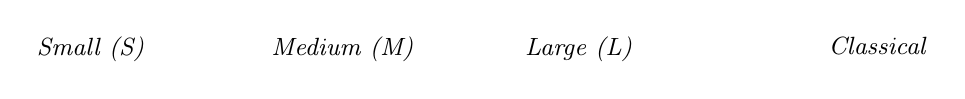
\begin{tikzpicture}
    \nimcirc{0}{0}{1}
    \nimcirc{0}{1}{1}
    \nimcirc{0}{2}{1}

    \nimcirc{0}{0}{2}
    \nimcirc{0}{1}{2}

    \nimcirc{0}{0}{3}
    \nimcirc{0}{1}{3}

    \node[below, font=\small] at (0.5,4) {\textit{Small (S)}};

    \nimcirc{3}{0}{0}
    \nimcirc{3}{1}{0}
    \nimcirc{3}{2}{0}

    \nimcirc{3}{0}{1}
    \nimcirc{3}{1}{1}
    \nimcirc{3}{2}{1}

    \nimcirc{3}{0}{2}
    \nimcirc{3}{1}{2}

    \nimcirc{3}{0}{3}

    \node[below, font=\small] at (3.7,4) {\textit{Medium (M)}};

    \nimcirc{6}{0}{0}
    \nimcirc{6}{1}{0}
    \nimcirc{6}{2}{0}
    \nimcirc{6}{3}{0}

    \nimcirc{6}{0}{1}
    \nimcirc{6}{1}{1}
    \nimcirc{6}{2}{1}

    \nimcirc{6}{0}{2}
    \nimcirc{6}{1}{2}
    \nimcirc{6}{2}{2}

    \nimcirc{6}{0}{3}

    \node[below, font=\small] at (6.7,4) {\textit{Large (L)}};

    \nimcircg{10}{0}{0}
    \nimcircg{10}{1}{0}
    \nimcircg{10}{2}{0}
    \nimcircg{10}{3}{0}
    \nimcircg{10}{4}{0}
    \nimcircg{10}{5}{0}
    \nimcircg{10}{6}{0}

    \nimcircg{10}{0}{1}
    \nimcircg{10}{1}{1}
    \nimcircg{10}{2}{1}
    \nimcircg{10}{3}{1}
    \nimcircg{10}{4}{1}

    \nimcircg{10}{0}{2}
    \nimcircg{10}{1}{2}
    \nimcircg{10}{2}{2}

    \nimcircg{10}{0}{3}

    \node[below, font=\small] at (10.5,4) {\textit{Classical}};

    \end{tikzpicture}
    \caption{Initial configurations for \textit{Nim}.} 
\end{figure}

\begin{figure}[H]
        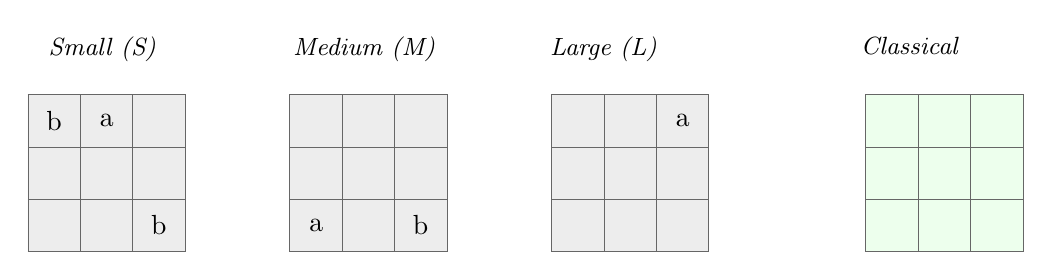
\begin{tikzpicture}[scale=0.95]
    \newcommand\x{0}
    \draw[step=0.7cm,draw=black!60,very thin,
    fill=black!7] (\x+0,0) grid (\x+2.1,2.1) rectangle (\x+0,0);
    \draw[thick] (\x+1.05,1.75) node{a};
    \draw[thick] (\x+1.75,0.35) node{b};
    \draw[thick] (\x+0.35,1.75) node{b};
    
    \node[below, font=\small] at (1,3) {\textit{Small (S)}};

    \newcommand\xx{3.5}
    \draw[step=0.7cm,draw=black!60,very thin,
    fill=black!7] (\xx+0,0) grid (\xx+2.1,2.1) rectangle (\xx+0,0);
    \draw[thick] (\xx+0.35,0.35) node{a};
    \draw[thick] (\xx+1.75,0.35) node{b};
    \node[below, font=\small] at (4.5,3) {\textit{Medium (M)}};
    
    
    \newcommand\xxx{7}
    \draw[step=0.7cm,draw=black!60,very thin,
    fill=black!7] (\xxx+0,0) grid (\xxx+2.1,2.1) rectangle (\xxx+0,0);
    \draw[thick] (\xxx+1.75,1.75) node{a};
    
    \node[below, font=\small] at (7.7,3) {\textit{Large (L)}};
    
    \newcommand\xxxx{11.2}
    \draw[step=0.7cm,draw=black!60,very thin,
    fill=green!07] (\xxxx+0,0) grid (\xxxx+2.1,2.1) rectangle (\xxxx+0,0);
    
    \node[below, font=\small] at (11.8,3) {\textit{Classical}};
    
    
\end{tikzpicture}
\caption{Initial configurations for \textit{TicTacToe}} 
    \label{nim_sample}
    \end{figure}


\subsection{Learning phase}

The learning phase of the evaluation consisted of computing the strategy for each approach. The strategies were computed for each initial state and saved for the next phase. We will proceed to interpret different aspects of the this process as well as the resulted strategies. 

\begin{minipage}{0.5\linewidth}
    \centering
    \begin{table}[H]
        \small
        \setlength{\tabcolsep}{0.5em}
        \def\arraystretch{1.1}
        \begin{threeparttable}
            \begin{tabular}{L{0.30\linewidth} p{0.09\linewidth}p{0.09\linewidth}p{0.1\linewidth}}
                \toprule[0.25mm]
                Approach & S & M & L
                \\
                \midrule[0.35mm]
                Minimax  & 390 & 4630 & 61023
                \\[20pt]
                Pruned minimax tree   & 83 & 347 & 2675
                \\[20pt]
                Pruned minimax rules & 35 & 85 & 283 
                \\
                \bottomrule[0.25mm]
            \end{tabular}
            \caption{Number of nodes in the computed tree for Nim}
        \end{threeparttable}
    \end{table}
\end{minipage}
\begin{minipage}{0.5\linewidth}
    \centering
    \begin{table}[H]
        \small
        \setlength{\tabcolsep}{0.5em}
        \def\arraystretch{1.1}
        \begin{threeparttable}
            \begin{tabular}{L{0.30\linewidth} p{0.09\linewidth}p{0.09\linewidth}p{0.1\linewidth}}
                \toprule[0.25mm]
                Approach & S & M & L
                \\
                \midrule[0.35mm]
                Minimax  & 896 & 7583 & 59704
                \\[20pt]
                Pruned minimax tree   & 105 & 73 & 2835
                \\[20pt]
                Pruned minimax rules & 109 & 61 & 2399 
                \\
                \bottomrule[0.25mm]
            \end{tabular}
            \caption{Number of nodes in the computed tree for TicTacToe}
        \end{threeparttable}
    \end{table}
\end{minipage}

The trees computed for the Minimax and the Pruned Minimax approaches are too large to be presented in this paper. Nevertheless, we can examine their structure by looking at the number of nodes in each tree. Such numbers are included in Figure 16 and their detailed values can be found in Tables 1 and 2. From those tables, we can notice the significant reduction in the tree size when using the pruning strategy compared to the full tree. As well as a further reduction by including the learned rules in the learning.

Unlike game trees, the weak constraints generated by the ILASP approach for each initial instance are concise and explainable. The strategy found for Nim (Figure 16), encode the mathematical strategy explained along with the game description. Lines 1, 2 and 3 define new predicates \texttt{nim\_sum/3} and \texttt{b/3} to save the \textit{Nim Sum} and the binary number of each digit for every pile, respectively. Using this new predicates, the weak constraint in line 4 penalizes an odd \textit{Nim Sum} for any digit. The strategy learned using the small instance only varies by penalizing \textit{nim\_sum(V0,V1,3)} instead of \textit{nim\_sum(V0,V1,4)}, this change is associated to the lack of counters on pile 4 for the small instance. 

The strategy found for TicTacToe with initial state \textit{M} (Figure 18) will give preference to stable models where there is a free space in a consecutive line, stated in line 1. A higher priority of 2 will be assigned to stable models where player $V0$, corresponding to the current player, completes a full line in the next state. This last fact encoded in lines 2 and 3, corresponds to the expected strategy of always choosing the action leading to a winning state. In the case of the initial state \textit{S} (Figure 17), lines 3 and 4 will penalize actions where the next state has a line with one cell taken and one free. Thus, encouraging actions that block the other player moves.  

\begin{center}
    \begin{lstlisting}[] 
nim_sum(V1,0,0) :- b(_,V1,_).
nim_sum(V1,V3+V2,V0) :- b(V0,V1,V2), nim_sum(V1,V3,V0-1).
b(V3,V1,V2) :- binary(V0,V1,V2), next(has(V3,V0)).
:~ nim_sum(V0,V1,4), V1\2 != 0.[1@1, 4, V0, V1]
    \end{lstlisting}
    \captionof{figure}{Strategy found by ILASP for Nim instances \textit{M} and \textit{L}}
\end{center}

\begin{center}
    \begin{lstlisting}[] 
:~ next(has(V0,V1)), in_line(V1,V2,V3).[1@1, 1, V0, V1, V2, V3]
:~ in_line(V0,V1,V2), next(free(V0)).[-1@2, 2, V0, V1, V2]
:~ next(has(V0,V1)), in_line(V2,V3,V1), 
   next(free(V2)).[1@2, 3, V0, V1, V2, V3]
:~ next(has(V0,V1)), next(has(V0,V2)), 
   next(has(V0,V3)), in_line(V1,V2,V3).[-1@2, 4, V0, V1, V2, V3]
    \end{lstlisting}
    \captionof{figure}{Strategy found by ILASP for TicTacToe instance \textit{S}}
\end{center}

\begin{center}
    \begin{lstlisting}[] 
:~ in_line(V0,V1,V2), next(free(V2)).[-1@1, 1, V0, V1, V2]
:~ next(has(V0,V1)), next(has(V0,V2)), 
   next(has(V0,V3)), in_line(V1,V2,V3).[-1@2, 2, V0, V1, V2, V3]
    \end{lstlisting}
    \captionof{figure}{Strategy found by ILASP for TicTacToe instance \textit{M}}
\end{center}



We present in Figure 16 the time taken by each approach to generate the strategy. These times are taking into account the saving process for each strategy, in the case of strategies in the form of trees, this process exported the tree into JSON format to provide faster access. The building times for ILASP include the generation of ordered examples from the Pruned Minimax approach as well as the ILASP process to compute the Hypothesis.

We notice how for the small TicTacToe the times for ILASP are considerably bigger than the rest. This overload is due to the abstraction process of ILASP, while the rest of the approaches can quickly compute a strategy for a small instance. For the medium size, we can notice that the Minimax approach takes the most time while Pruned Minimax learning rules takes the least time. This behavior correlates with the number of explored nodes. For the larger instance, there are some key points to notice. First, we can see how the game of Nim behaves as it does for the medium size with Pruned Minimax, whereas for TicTacToe we can see a drastic change. In the case of ILASP no strategy was found to cover all the ordered examples. 
% The examples that provoked it were those referring to earlier stages of the game where a clear strategy is hard to find even for a human. Such cases must see over 2 steps into the future to make the decision. 
Pruned Minimax with rules outperformed the rest of the approaches in almost every configuration, while for the large TicTacToe instance we can see a bad performance.
% We can attribute this increase in time to the lack of abstraction used for the game. The rules generated for this game consist of only constants and only abstract players, unlike the ones presented for Nim where the pile numbers are substituted by variables. As a result, the number of rules for the strategy increases, generating over 1000 rules that are included in each call to \textit{clingo} slowing down its response. 

\begin{figure}[H]
    \centering
    \includegraphics[width=\linewidth]{bar_build.pdf}
    \caption{Learning times for each approach. The bar colors are computed applying $log_{10}$ to the proportion of nodes, with 100 being the tree with the most nodes for each game and size.}
\end{figure}

\subsection{Approaches against Random-Agent}

For each learning approach, we created an agent with the capability to choose an action in the current state of the game $s_c$. This judgment is based on the generated strategies during the learning phase. Table 3 gives a summary of how each agent will select an action during gameplay. 

\begin{table}[H]
	\centering
	\small
	\setlength{\tabcolsep}{0.5em}
	\def\arraystretch{1.1}
	\begin{threeparttable}
		\begin{tabular}{L{0.15\linewidth} p{0.25\linewidth} p{0.5\linewidth}}
			\toprule[0.25mm]
            Agent & Strategy & Action selection for current state $s_c$ 
            \\
			\midrule[0.35mm]
            Minimax  & Full minimax tree 
            &Finds a node in the tree with for state $s_c$ and choose the action corresponding to the children which maximizes the score. If no node is found for $s_c$, choose a random action.
            \\[20pt]
            Pruned minimax tree   & Pruned minimax tree 
            & Same as Minimax agent. The unexplored sections of the tree will increase the likelihood of $s_c$ not being part of the tree.
            \\[20pt]
            Pruned minimax rules & ASP rules   
            & Includes the rules as part of the clingo call and selects one of the remaining stable models. 
            \\[20pt]
            ILASP & Weak constraints  
            & Includes the weak constrains as part of the clingo call and selects the optimal stable model.
            \\
			\bottomrule[0.25mm]
		\end{tabular}
		\caption{Tabular summary of learned strategies}
	\end{threeparttable}
\end{table}

\begin{figure}[H]
    \centering
    \includegraphics[width=\linewidth]{bar_vs.pdf}
    \caption{Number of winning matches for each approach against a random agent including their mean response time.}
\end{figure}

We played each agent against a Random-Agent and compared the number of wined matches in Figure 20. Using the classical initial state, we simulated a total of 300 matches switching the starting player in each game to avoid an initial advantage to either player. 

We can see that out of all approaches that learned from small instances, only the ILASP strategy was able to outperform the random agent in TicTacToe. This behavior continued throughout the experiment showing the potential of ILASP to generalize into bigger instances. For the game of Nim, the Pruned Minimax agent working with rules was also able to generalize and wan against the random agent in over 75\% of the matches. We can also notice a slight improvement when using the full Minimax tree instead of the pruned tree in both games. Regarding the response times, it is easy to notice the increment on response times for indexing the tree. While, on the other hand, adding more information to the encoding showed to provide a fast response.

\subsection{Framework}

In addition to the research performed on these approaches, we made available a generalized framework. With this framework, we want to encourage the use and research of ASP in two-player games. Our implementation allows simple expansions for new games following the GLD formalisms as well as new approaches for learning strategies. These expansions will automatically generate the command-line tools to build strategies, create agents and compute benchmarks. We also make available the tree visualizations by simply defining an ASCII representation of the states for the new game. The code can be found in \href{https://github.com/atreyasha/asp-game-strategies}{github}\footnote{https://github.com/susuhahnml/asp-game-strategies}, including a detailed explanation of how to extend it with new games and approaches. 



\section{Discussion}
\label{discussion}

A deeper analysis of the results showed different issues and advantages in each approach taken. Computing the full Minimax tree showed to be generally inefficient. We can see an expected exponential blowup in the number of nodes that correlates with the computation and response times. This outcome was expected as it is related to the brute-force nature of the algorithm. By pruning the tree we notice a clear improvement in the number of nodes. This improvement will also depend on the specific instance and the ordered in with actions are explored. It was due to this random factor that the algorithm was able to skip a big part of the tree in the medium TicTacToe instance, leading to fewer nodes than the ones from the small instance. Even though the pruning had better overall run times and improved space, the contrasting outcome can be seen in the slight difference in performance during gameplay. We can attribute this decrease on winned games, compared to plain Minimax, to the cases where the gameplay falls into the unexplored states of the pruned tree resulting in a random action instead of an informed one.

By learning ASP rules that abstracted the Pruned Minimax tree, we can notice an improvement in the scalability and the number of nodes. This improvement, however, was not the same for both games. By analyzing Figure 20 we can notice a very good performance for Nim, but a poor one for TicTacToe. This can be attributed to the level of abstraction in the rules generated for each game. In TicTacToe strategy rules consist of only constants except for the player's names, whereas the ones presented for Nim, the pile numbers are also substituted by variables. This result can also be seen in the increased build time for the larger instance of TicTacToe. In this case, the number of rules for the strategy increases, generating over 1000 rules that are included in each call to \textit{clingo} slowing down its response. 


Learning weak constraints with ILASP successfully generalized from small instances into the real game. However, it was not able to reach a conclusive strategy for the large instance of TicTacToe. We noticed that examples provoking this outcome were those referring to earlier stages of the game where a clear strategy is hard to find even for a human; such cases must see over 3 steps into the future to make the decision. The advantage that ILASP provided with explainable and simple strategies can arguably be outweighed by the complexity of the language bias. While the language bias for TicTacToe was intuitive, the one for Nim had to be carefully handcrafted based on previous knowledge of the expected strategy. 

\section{Conclusions}
\label{conclusions}
With this project we were able to learn different strategies for two-player games. We defined a novel variant of the Minimax algorithm which makes use of optimization statements to speed the computation by pruning parts of the game tree. This technique also showed to be good at generalizing for bigger instances when symmetries in the game can be enforced. Even though the strategy it generates as ASP rules can be interpreted by a human, it is not as concise and generalizable as the one learned using ILASP.

Employing Inductive Logic Programming with ILASP system helped us find explainable and scalable strategies. We believe this could be further investigated to tackle some of the downsides of the approach by using of its feature for noisy examples. If we add a weight factor to each example depending on how certain it is of the outcome of the game, we could prioritize strategies in the last stages of the game.

By representing the games with GDL and computing the game dynamics using ASP we created a generalized framework that facilitates the inclusion of new games and techniques for further research. In this project we separated the generation of the strategies for the gameplay. It would also be interesting to explore the option of performing computations during gameplay to improve on the existent strategies.

\newpage
\addcontentsline{toc}{section}{References}
\bibliographystyle{apalike}
\bibliography{bibtex}
\nocite{*}
\end{document}